\chapter{System Design}

\section{System Architecture}
ByteVault follows a three-tier, multi-node architecture. The Next.js frontend acts as the presentation layer. The Bun/Express backend serves as the business logic and transaction coordinator. The data layer consists of two independent PostgreSQL databases. To facilitate cross-branch reads, the Main DB uses a Foreign Data Wrapper (FDW) to map tables from the Sub DB. For writes, the Backend directly coordinates a Two-Phase Commit (2PC) between both databases.

\section{Database Design}
The relational schema enforces strict integrity. 
\subsection{Core Entities}
\begin{itemize}
    \item \textbf{Users \& Accounts:} Customers and their associated branch accounts.
    \item \textbf{Journal Entries \& Lines:} The double-entry ledger where \texttt{SUM(amount\_cents) = 0}.
    \item \textbf{Transfer Requests:} Workflow tables linking to \texttt{account\_holds} to freeze funds during pending approvals.
    \item \textbf{Audit Logs:} Time-series records of all system actions.
\end{itemize}

\begin{landscape}
\begin{figure}[p]
    \centering
    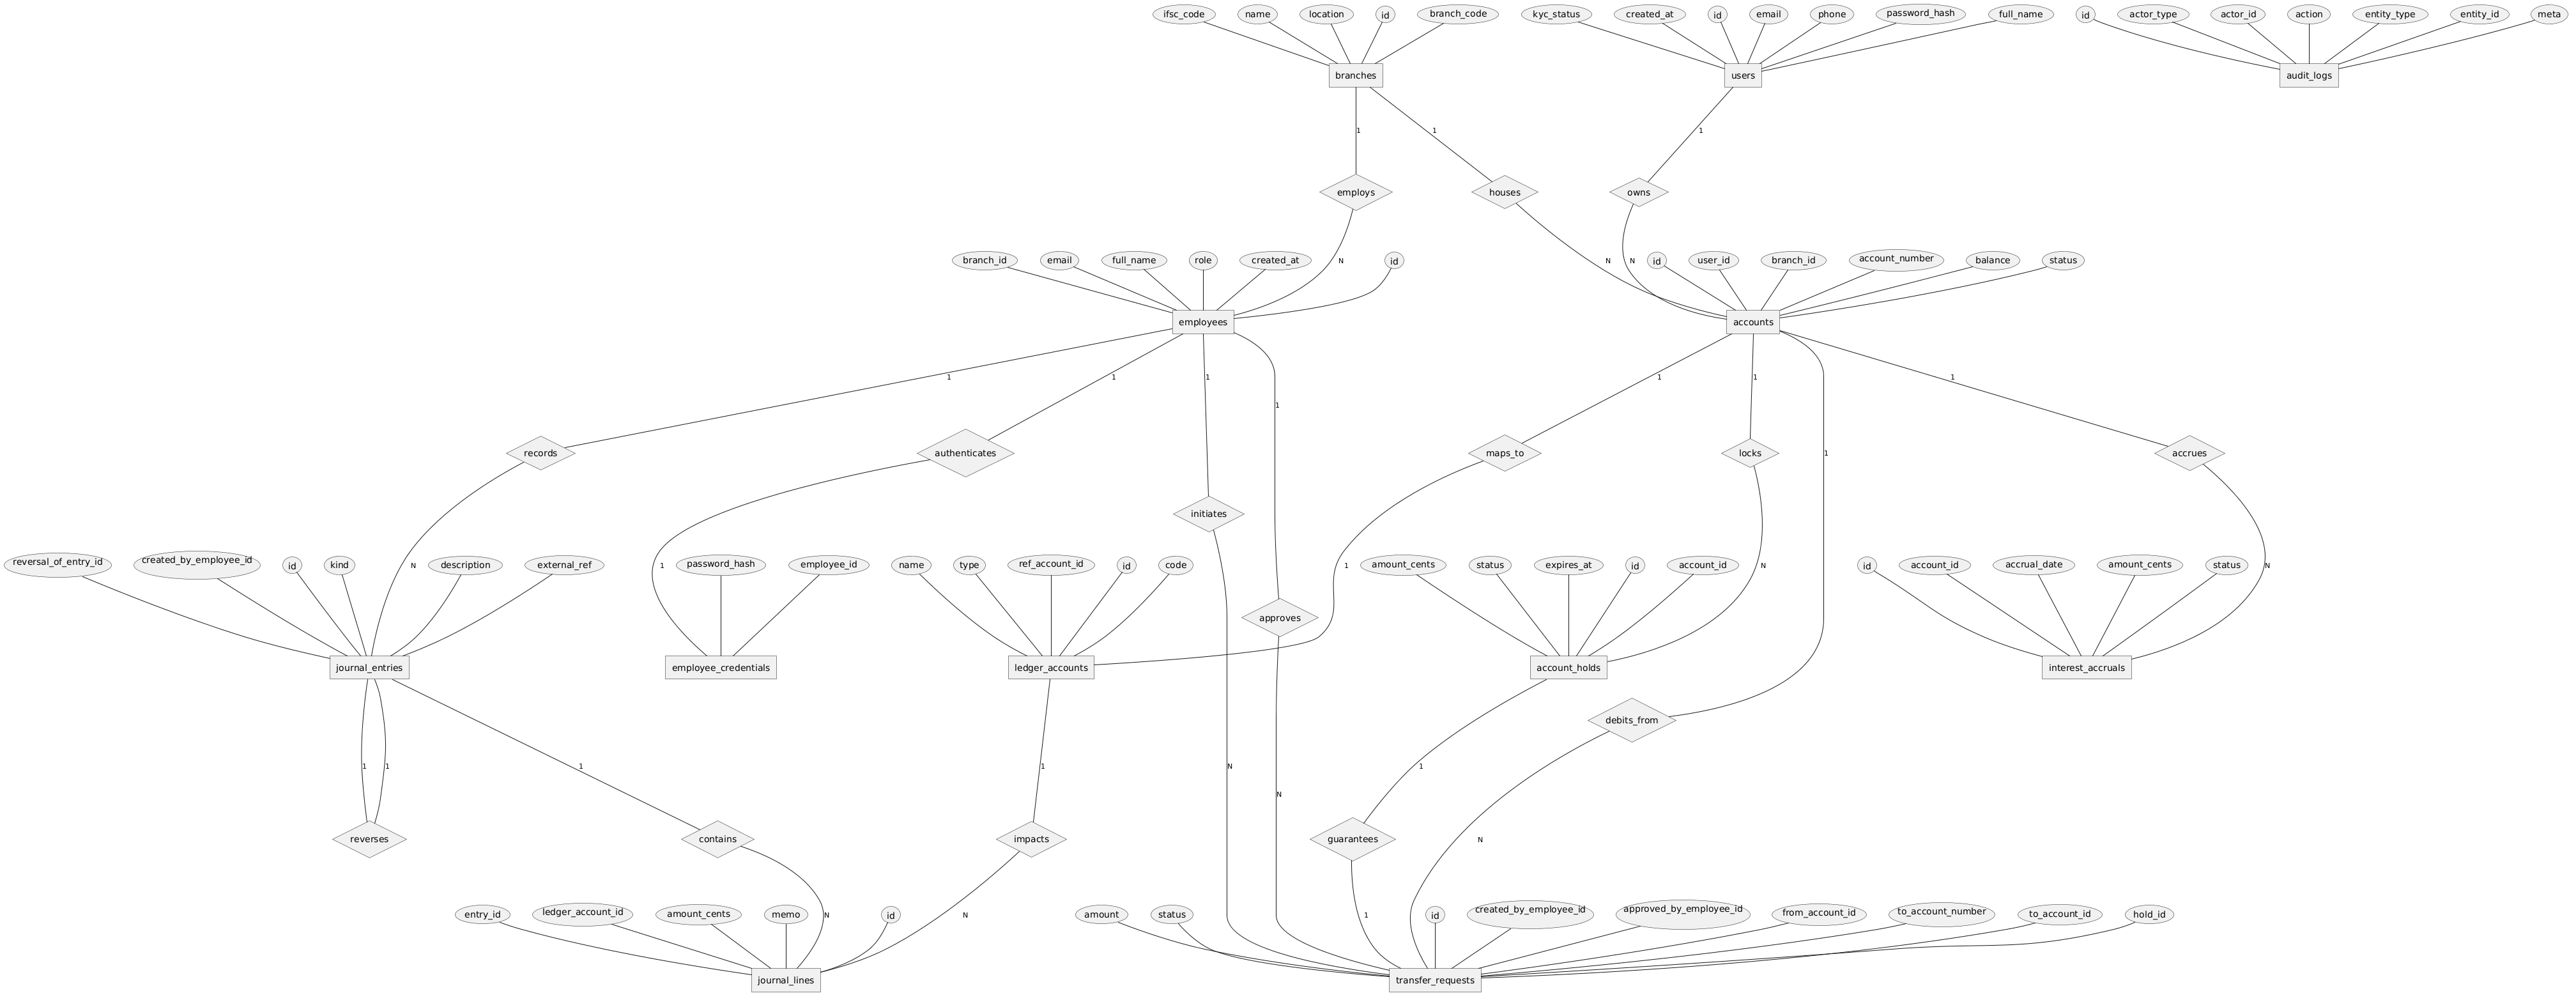
\includegraphics[width=1.2\linewidth,height=0.8\textheight,keepaspectratio]{figures/ERD.png}
    \caption{ByteVault Entity Relationship Diagram (ERD)}
    \label{fig:erd}
\end{figure}
\end{landscape}

\section{Security Aspects}
\begin{itemize}
    \item \textbf{Stateless Authentication:} JWTs are used for employee sessions, explicitly embedding branch routing and Role-Based Access Control (RBAC).
    \item \textbf{Idempotency:} All payment routes require an \texttt{Idempotency-Key} to prevent duplicate charges resulting from network retries.
    \item \textbf{Audit Trail:} A highly integrated logging service captures the actor UUID, entity, and JSON metadata for every state mutation.
\end{itemize}

\section{Performance Aspects}
\begin{itemize}
    \item \textbf{Circuit Breakers:} FDW queries utilize strict \texttt{statement\_timeout} configurations so a downed remote branch does not indefinitely hang the main API.
    \item \textbf{Materialized Views:} Ledger balances are aggregated into daily materialized views to prevent expensive recalculations of the entire journal history. These are refreshed concurrently during EOD batch jobs.
    \item \textbf{Batch Processing Logic:} Heavy calculations (interest accrual) are offloaded to admin-triggered batch jobs with optimistic concurrency control (FOR UPDATE) to prevent double-posting.
    \item \textbf{Connection Pooling:} Efficient handling of concurrent database connections using the \texttt{pg} driver.
\end{itemize}
